\documentclass[10pt,a4paper]{article}

\usepackage{natbib}
\usepackage{graphicx}
\usepackage{color}
\usepackage{amsmath} 
\usepackage{amssymb} 
\usepackage{bm} 
\usepackage{hyperref}
\usepackage{tikz}

\voffset -0.5in
\oddsidemargin 0.2in
\textheight 24cm
\textwidth 6in
\linespread{1}

\newcommand\xqed[1]{%
  \leavevmode\unskip\penalty9999 \hbox{}\nobreak\hfill
  \quad\hbox{#1}}
\newcommand\demo{\xqed{$\triangle$}}

\newcommand{\red}{\textcolor{red}}
\newcommand{\blue}{\textcolor{blue}}

\newcommand{\expect} {{\mathbb{E}}}
\newcommand{\pt} {\tilde{p}}
\newcommand{\nei} {\textrm{ne}}
\newcommand{\alphat} {\tilde{\alpha}}
\newcommand{\betat} {\tilde{\beta}}
\newcommand{\pb} {\bar{p}}
\newcommand{\kappab} {{\boldsymbol{\kappa}}}
\newcommand{\thetab} {{\boldsymbol{\theta}}}
\newcommand{\Thetab} {{\boldsymbol{\Theta}}}
\newcommand{\varthetab} {{\boldsymbol{\vartheta}}}
\newcommand{\Yset} {\mathcal{Y}}
\newcommand{\Xset} {\mathcal{X}}
\newcommand{\intd} {\textrm{d}}
\newcommand{\phib} {\boldsymbol{\phi}}
\newcommand{\gammab} {\boldsymbol{\gamma}}
\newcommand{\mub} {\boldsymbol{\mu}}
\newcommand{\Sigmawinv} {{\boldsymbol{\it \Sigma}}_w^{-1}}
\newcommand{\Sigmamat} {{\boldsymbol{\it \Sigma}}}
\newcommand{\Upsilonmat} {{\boldsymbol{\it \Upsilon}}}
\newcommand{\Lambdamat} {{\boldsymbol{\it \Lambda}}}
\newcommand{\Gammamat} {{\boldsymbol{\it \Gamma}}}
\newcommand{\Pimat} {{\boldsymbol{\it \Pi}}}
\newcommand{\Amat} {\textbf{\textit{A}}}
\newcommand{\Bmat} {\textbf{\textit{B}}}
\newcommand{\Cmat} {\textbf{\textit{C}}}
\newcommand{\Dmat} {\textbf{\textit{D}}}
\newcommand{\Gmat} {\textbf{\textit{G}}}
\newcommand{\Kmat} {\textbf{\textit{K}}}
\newcommand{\Lmat} {\textbf{\textit{L}}}
\newcommand{\Mmat} {\textbf{\textit{M}}}
\newcommand{\Qmat} {\textbf{\textit{Q}}}
\newcommand{\Pmat} {\textbf{\textit{P}}}
\newcommand{\Rmat} {\textbf{\textit{R}}}
\newcommand{\Tmat} {\textbf{\textit{T}}}
\newcommand{\Zmat} {\textbf{\textit{Z}}}
\newcommand{\Qt} {\widetilde{\textbf{\textit{Q}}}}
\newcommand{\Qtinv} {\widetilde{\textbf{\textit{Q}}}^{-1}}
\newcommand{\Imat} {\textbf{\textit{I}}}
\newcommand{\Hmat} {\textbf{\textit{H}}}
\newcommand{\Vmat} {\textbf{\textit{V}}}
\newcommand{\Umat} {\textbf{\textit{U}}}
\newcommand{\bvec} {\textbf{\textit{b}}}
\newcommand{\dvec} {\textbf{\textit{d}}}
\newcommand{\evec} {\textbf{\textit{e}}}
\newcommand{\kvec} {\textbf{\textit{k}}}
\newcommand{\tvec} {\textbf{\textit{t}}}
\newcommand{\xvec} {\textbf{\textit{x}}}
\newcommand{\yvec} {\textbf{\textit{y}}}
\newcommand{\zvec} {\textbf{\textit{z}}}
\newcommand{\wvec} {\textbf{\textit{w}}}
\newcommand{\vvec} {\textbf{\textit{v}}}
\newcommand{\svec} {\textbf{\textit{s}}}
\newcommand{\gvec} {\textbf{\textit{g}}}
\newcommand{\fvec} {\textbf{\textit{f}}}
\newcommand{\rvec} {\textbf{\textit{r}}}
\newcommand{\mdot} {\dot{m}}
\newcommand{\hdot} {\dot{h}}
\newcommand{\hdotb} {\boldsymbol{\dot{h}}}
\newcommand{\muvec} {\boldsymbol{\mu}}
\newcommand{\tr} {\textrm{tr}}
\newcommand{\Psix} {{\boldsymbol{\it \Psi}}_{\xvec}}
\newcommand{\Phimat} {{\boldsymbol{\it \Phi}}}
\newcommand{\Psitheta} {{\boldsymbol{\it \Psi}}_{\varthetab}}
\newcommand{\Psia} {{\boldsymbol{\it \Psi}}_{A}}
\newcommand{\Psixinv} {{\boldsymbol{\it \Psi}}_{\xvec}^{-1}}
\newcommand{\vvm} {\boldsymbol {\mathcal \upsilon}}
\newcommand{\upsilonb} {\boldsymbol {\upsilon}}
\newcommand{\alphab} {\boldsymbol {\alpha}}
\newcommand{\zetab} {\boldsymbol {\zeta}}
\newcommand{\betab} {\boldsymbol {\beta}}
\newcommand{\zerob} {\boldsymbol {0}}
\newcommand{\oneb} {\boldsymbol {1}}
\renewcommand{\Re} {\mathbb {R}}

\bibliographystyle{harvard}	
%

\title{Physical-statistical techniques, data-feature assimilation and source separation in environmental applications}
\author{Andrew, Bill, Botond and Jonty}


\makeatletter
\renewcommand\section{\@startsection{section}{1}{\z@}%
                                  {-3.5ex \@plus -1ex \@minus -.2ex}%
                                  {2.3ex \@plus.2ex}%
                                  {\normalfont\large\bfseries}}
\makeatother


\begin{document}

\maketitle

\begin{abstract}
Several methods for assimilating data with numerical model outputs have been proposed and today these methods are at the core of several data-model fusion approaches in the environmental sciences. This paper serves a dual scope. The first aim is to review several of these methods by categorising in three groups according to the way in which the numerical model outputs feature in the model. The second aim is to present and discuss in detail a fourth, rather less known category which we refer to as data-feature assimilation. In data-feature assimilation, features elicitated from numerical models are the sole integration constraint within a predominantly data-driven framework and is of use when the structural discrepancy in numerical models is hard or impossible to characterise. We consider four types of feature assimilation (i) frequency characteristics (ii) spatial shcaracteristics (iii) dynamic evolution and (iv) natural constraints, the first three of which have featured implicitly in some of the literature. %We employ data-feature assimilation on toy numerical models and show how, combined, this approach facilitates inference in a challenging, ill-posed application, where only process superpositions are observed. Data-feature assimilation is finally applied to the Antarctic ice sheet, where height loss due to surface mass balance and ice dynamics is estimated solely from altimetry observations.
\end{abstract}


\section{Introduction}

Data for use in environmental studies stems from two sources: (i) numerical models (simulators) and (ii) observations. Technological advances over the past decades have allowed both sources to generate larger and more complex data, aimed ultimately for the analysis and possibly prediction in important application areas such as ecology, climate change and public health. Typically the analyst tasked with using the data is required to simultaneously use multiple numerical model outputs, and observations from sources as diverse as satellite and underground sensors in order to maximise the information content of results (which could be inferences on physical model calibration parameters, stochastic model parameters or predictions) in a process known as data assimilation. There are two critical caveats to this process. (i) it has frequently become computationally prohibitive to retain all generated data and model output runs within a traditional assimilation framework and (ii) despite the all-time high numerical model resolutions employed, model outputs contain structural uncertainties and biases which are hard to quantify. These two issues, exacerbated by increased data and computational availability, are forcing an ongoing development in data-model integration strategies and generating a need for pragmatic approaches which allow analysts to maximise information use as efficiently as possible.

All approaches developed to tackle model-integration, make various (sometimes implicit) assumptions about numerical model validity and the role the outputs should play in the inference. Whilst all assume that the numerical model is informative of the underlying system, the degree to which this is so varies. It is important to be aware of the different methods available, at least at a conceptual level, lest the potential of the data and the model outputs are not maximised to the full. The first purpose of this paper is to give a broad account of the methods available. We start in Section 2 by discussing the three most common approaches to data-model integration (i) the mechanistically-motivated approach, (ii) the model-informed prior approach, and (iii) the multi-level observation appraoch, and discuss the benefits and applicability of each of these appraoches.

The second purpose is to formalise a fourth, less frequented method which we term the data-feature assimilation approach in Section 3. In this  approach, numerical model outputs are not used \emph{talis qualis}, rather \emph{characteristics}  of the outputs extracted through expert elicitation and which, subject to some probability, are deemed to be representative of the physical system. Disregarding characteristics of numerical outputs which are subject to structural uncertainty (for example certain spatial features or problematic areas) serves a dual purpose of obviating the need to define the statistics of the discrepancy while inflating uncertainty due to the omission of this term.  In Section 4 we see how this method may be used to solve a challenging problem in several application areas, that of observed superpositions before applying it to a real case study, that of the Antarctic ice sheet. Section 5 concludes the work.

%This method is seen to solve the issues presented in the first paragraph directly. (i) Several simulation runs or emulation are typically not necessary since summary characteristics are used instead of the simulator outputs. This  reduces the effective data size in assimilation without promoting information loss. (ii) Expert knowelege is used to disregard characteristics of numerical outputs which are subject to structural uncertainty (for example certain spatial features or problematic areas). This serves the dual purpose of obviating the need to define the statistics of the discrepancy while inflating uncertainty due to the omission of this term.

 
%The second issue is particularly problematic as it hinders realistic uncertainty assessment. Uncertainties in simulation which arise due to parametric unknowns such as initial/boundary conditions and errors due to solver resolution may be catered for, for instance through the framework of Goldstein and Rougier, 2008. When there is not sufficient expert knowledge to characterise the structural discrepancy between the simulator and the real world (or sufficient statistics of this discrepancy) one is forced to resort to solely qualitative descriptions of the model in assimilation. This is because one may not (strictly) alter any structural description of a simulator with data which is subsequently used for assimilation.  This major difficulty obstruct quantification of misrepresentation with negative implications on our uncertainty judgements. 


\section{Assimilation of numerical models and physical observations: state of the art}

In this section we review three of the most widely used categories of Bayesian data-model assimilation. For illustration the independent variable is omitted throughout; typically the process is multivariate, temporally and/or spatially dependent. 

\subsection{The mechanistically motivated stochastic model}

The first and most direct way of incorporating numerical models within a stochastic framework for assimilation, is to add stochastic terms to the deterministic model to account for uncertainty (both parametric and structural). The deterministic component can either be left unchanged, or instead (and most frequently) simplified either by ignoring complicated physics, using linearity assumptions or by using a simple, coarse discretisation \citep{Berliner_2003}. The parameters in the numerical model (with physical intepretation) frequently appear in the stochastic equivalent and may be estimated directly. 

Let $y$ denote the process, $z_o$ physical observations, $\theta_o$ parameters describing the observation error characteristics and $\theta_p$ parameters within the stochastic mechanistically motivated model. The framework employed in this scenario is the standard hierarchical framework \citep[e.g.][]{Wikle_2003} which defines conditional models on three layers:
\begin{itemize}
\item Level 1: Observation model: $p(z_o | y, \theta_o)$
\item Level 2: Process model: $p(y | \theta_p)$
\item Level 3: Parameter model: $p(\theta_o, \theta_p)$
\end{itemize}
\noindent Hierarchical models like this one provide a neat way to reduce a complex model into three simpler ones, linked together through conditional dependencies which we depict through the following graphical model:

\begin{figure}[h!]
\centering
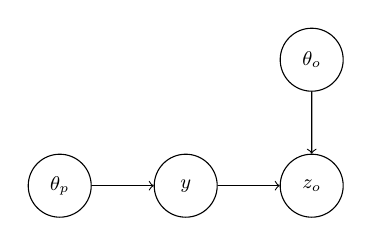
\begin{tikzpicture}[scale=0.8,every node/.style={transform shape}]
%[inner sep=1mm] 
[line width=1pt]
\path (0,0) node (thetap) [shape=circle,minimum size=1cm,draw] {\small $\theta_p$};
\path (2,0) node (y) [shape=circle,minimum size=1cm,draw] {\small $y$};
\path (4,0) node (zo) [shape=circle,minimum size=1cm,draw] {\small $z_o$};
\path (4,2) node (thetao) [shape=circle,minimum size=1cm,draw] {\small $\theta_o$};

\draw [->] (thetap) to (y);
\draw [->] (y) to (zo);
\draw [->] (thetao) to (zo);
\end{tikzpicture}
\end{figure}

\noindent In this case no numerical model outputs are needed, as the prior process model $y$ is deemed to be sufficiently representative such that simulator model outputs $z_m$ would not provide any further information about the process model, i.e. $p(y | \theta_p,z_m) \approx p(y | \theta_p)$. The object of interest $p(y|z_o)$ is found by applying Bayes theorem and marginalising out the unknown parameters:
\begin{equation}
p(y|z_o) \propto \iint p(z_o | y, \theta_o)p(y | \theta_p)p(\theta_o, \theta_p) \intd \theta_p \intd\theta_o
\end{equation}

In the mechanistically motivated approach, an instance of \emph{science-based parameterization} \citep{Leeds_2012}, the numerical model is deemed to be faithful to the true process, and thus able to reproduce the emergent phenomena. This approach can thus only be used when there exists a model which is sufficiently simple and yet realistic to define the Level 2 process model. This is the case in several applications.  In \cite{Hooten_2008}, for example, the numerical model is Fisher's reaction-diffusion equation whilst the stochastic model is the finite-differenced, explicit Euler discrete equivalent. Similarly, a process model derived from heat equation is used for paleoclimate temperature reconstruction by \cite{Brynjarsdottir_2011}. In \cite{Wikle_2001}, the simplified model is the set of linear shallow-water equations subsequently reduced in dimensionality using an orthogonal basis set. In \cite{Berliner_2003b} air-sea interactions are studied through stochastic, simplified atmospheric and quasi-geostrophic ocean models. In \cite{Milliff_2011} a process model for the vector winds is based on approximations to the Rayleigh friction equation. 


In many cases a mechanistic-motivated model is not self-evident, particularly when what is termed the \lq process model\rq~is actually just one physical process influenced by several others within a complex network of models. In such cases no simple structure for the process model exists. The first alternative is a fully data-driven approach where numerical models are ignored entirely. The second, discussed next, is to integrate the physical model as is within the framework.


\subsection{The model-informed prior}\label{sec:mip}

The model-informed prior approach is similar to the previous case, in that one attempts to configure the process model based on available science, with the difference that numerical model outputs are used to reduce uncertainty on the process model: the numerical model \emph{structure} itself is not of direct use.  Here thus, the process model in the hierarchial framework is one which is able to reconstruct the uncertainty of the physical (deterministic) simulator through uncertainties in simulator inputs and parameters, which could refer to anything from boundary conditions to forcings to solver resolution \citep{Goldstein_2009}. Structural discrepancy in this framework is catered for through a discrepancy term $\delta$ which is estimated by comparing the observations to the model outputs \citep{Kennedy_2001}.

Denote the process as  $y \in \mathcal{Y}$ (including past, present and future states) and an imperfect simulator of $y$ as $f(\vartheta_m)$, $\vartheta_m \in \Theta_m$. The process model is then the simulator evaluated at some \emph{best input} $\theta_m \in \Theta_m$ with an added discrepancy $\delta$. It is important to realise the difference between the variable $\vartheta_m$ which indexes $\Theta_m$ and $\theta_m$ which is a random variable over the same space: $f(\vartheta_m)$ is a function mapping $\Theta_m$ to $\mathcal{Y}$, whilst $f(\theta_m)$ is another random variable taking values in $\mathcal{Y}$, the distribution of which is fully governed by that of $\theta_m$ (the study of $f(\theta_m)$ is termed \emph{uncertainty analysis} \cite{OHagan_1998}). For example, imagine that $f(\vartheta_m)$ produces an air pollution map subject to a pollutant source location $\vartheta_m$. We can clearly produce as many maps as we wish to by indexing through $\vartheta_m$, and sometimes we want to characterise this relationship (see Emulation later), however the process $y^*$ is defined to be $f(\cdot)$ evaluated at $\theta_m$, and we generally would like to find a posterior distribution over $\theta_m$ too. 

Returning to the process model, as alluded to earlier the inaccuracy in the simulator is compensated for with the use of a discrepancy term $\delta$ so that
\begin{equation}
y^* = f(\theta_{m}) + \delta,
\end{equation}
\noindent which, if given as $\delta \sim \mathcal{N}(\mu_\delta,\Sigma_\delta)$, induces the conditional distribution 
\begin{equation}
p(y^* | \theta_m, \theta_\delta) = \mathcal{N}(f(\theta_m) + \mu_\delta, \Sigma_\delta)
\end{equation}
\noindent The discrepancy term, although not discussed here, plays a crucial role in the framework \citep{Brynjarsdottir_2013}. In general $\delta$ may also be dependent on $\theta_m$ and there are several ways, not reviewed here, to tackle this problem \citep[e.g.][]{Rougier_2007}. 
%It is important to stress the here $\theta^*$ is the unknown (we will place a prior over $\theta^*$) and $\theta_m$ should be treated as independent variables on an extended domain. The unknown appears in the constraint which is not standard. However 
%this equation leads to a simple conditional distribution if $y$ is a deterministic function of $\theta_m$ (i.e. $y$ is fully defined by $\theta_m$, as is the case with deterministic simulators) since then, for $\theta_m = \theta^*$ (and ignoring $\delta$ for the time being), $p(y | \theta^*) = \delta(y - y(\theta^*))$ so that 
%\begin{equation}
%p(y^* | \theta^*) = \int p(y^*|y)p(y | \theta^*) \intd y = p(y^* | y(\theta^*))
%\end{equation}
%\noindent which explicitly shows the relationship between $y^*$ and $\theta^*$ and is invariably a very complicated distribution. 
The ensuing graphical model for this setup is as follows
\begin{figure}[h!]
\centering
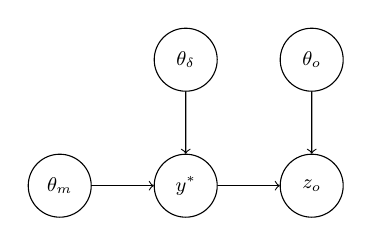
\begin{tikzpicture}[scale=0.8,every node/.style={transform shape}]
%[inner sep=1mm] 
[line width=1pt]
\path (2,0) node (thetam) [shape=circle,minimum size=1cm,draw] {\small $\theta_m$};
\path (4,0) node (ystar) [shape=circle,minimum size=1cm,draw] {\small $y^*$};
\path (6,0) node (zo) [shape=circle,minimum size=1cm,draw] {\small $z_o$};
\path (6,2) node (thetao) [shape=circle,minimum size=1cm,draw] {\small $\theta_o$};
\path (4,2) node (thetad) [shape=circle,minimum size=1cm,draw] {\small $\theta_\delta$};

\draw [->] (thetam) to (ystar);
\draw [->] (ystar) to (zo);
\draw [->] (thetao) to (zo);
\draw [->] (thetad) to (ystar);
\end{tikzpicture}
\end{figure}

\noindent This is once again the 3-layer hierarchical model but with the unknown parameters $\theta_m$ actual \emph{physical} parameters appearing within a deterministic model. The required posterior $p(y^* | z_o)$ is estimated by marginalising out all the nuisance variables
\begin{equation}\label{eq:Sim_simple}
p(y^*|z_o) \propto \iint p(z_o | y^*, \theta_o)p(y^* |\theta_m, \theta_\delta)p(\theta_o, \theta_m, \theta_\delta) \intd \theta_m \intd\theta_o \intd\theta_\delta
\end{equation}

The problem with this setup, as discussed in \citep{Higdon_2004}, is that evaluating $p(y^* | \theta_m, \theta_\delta)$ for some $\theta_m$ is expensive (unless $f(\cdot)$ is very simple which is rarely the case). One would need to evaluate $f(\theta_m)$ repeatedly (for different values of $\theta_m$) which is  prohibitive in complex systems. Strategic choices for $\theta_m$ for making the integral in (\ref{eq:Sim_simple}) easier are given in \cite{Rougier_2007}. One other choice is to use the samples to approximate this as a Gaussian distribution as discussed in Example 1 of Appendix A (Extended Kalman filtering).


\demo


\subsubsection*{Emulation}

Emulation is an extension of the basic model-informed prior approach for when $f$ is too complex to evaluate repeatedly. In emulation we consider the presence of a secondary stochastic process $y$ which expresses a simple probabilistic relationship between $\vartheta_m$ and $y^*$. In particular, if a simple linear relationship can be found for $y = f(\vartheta_m)$ (for example, $y = \beta\vartheta_m + e_y$) as we shall see later huge simplifications are possible. Formulating $y$ as a stochastic model over $\vartheta_m$ is a procedure known as \emph{emulation}. The model outputs $z_m$ can now be considered as \emph{realisations} of $y$ at different points of $\vartheta_m$ (whereas before, they were one-to-one mappings of $\theta_m$). The effect is an added process layer in the hierarchical framework (parameterised through $\theta_p$) as follows:

\begin{figure}[h!]
\centering
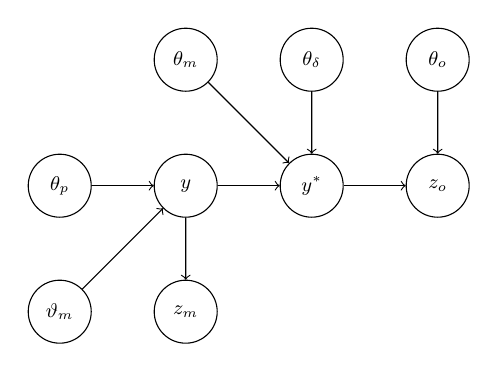
\begin{tikzpicture}[scale=0.8,every node/.style={transform shape}]
%[inner sep=1mm] 
[line width=1pt]
\path (2,2) node (thetam) [shape=circle,minimum size=1cm,draw] {\small $\theta_m$};
\path (0,0) node (thetap) [shape=circle,minimum size=1cm,draw] {\small $\theta_p$};
\path (2,0) node (y) [shape=circle,minimum size=1cm,draw] {\small $y$};
\path (4,0) node (ystar) [shape=circle,minimum size=1cm,draw] {\small $y^*$};
\path (6,0) node (zo) [shape=circle,minimum size=1cm,draw] {\small $z_o$};
\path (6,2) node (thetao) [shape=circle,minimum size=1cm,draw] {\small $\theta_o$};
\path (4,2) node (thetad) [shape=circle,minimum size=1cm,draw] {\small $\theta_\delta$};
\path (2,-2) node (zm) [shape=circle,minimum size=1cm,draw] {\small $z_m$};
\path (0,-2) node (vartheta) [shape=circle,minimum size=1cm,draw] {\small $\vartheta_m$};

\draw [->] (thetap) to (y);
\draw [->] (thetam) to (ystar);
\draw [->] (y) to (ystar);
\draw [->] (ystar) to (zo);
\draw [->] (thetao) to (zo);
\draw [->] (thetad) to (ystar);
\draw [->] (y) to (zm);
\draw [->] (vartheta) to (y);
\end{tikzpicture}
\end{figure}

\noindent Note that $y$ is only related to $\theta_m$, the best input, through $y^*$ ($y$ itself is simply a stochastic model on $\vartheta_m$ which provides no information on $\theta_m$).

On one hand, emulation simplifies things considerably since the required posterior distribution is now found as 
\begin{equation}
p(y^*|z_o,z_m,\vartheta_m) \propto \iint p(z_o | y^*, \theta_o)p(y^* | \theta_\delta, y,\theta_m)p(z_m | y)p(y | \theta_p,\vartheta_m)p(\theta^*,\theta_o, \theta_p, \theta_\delta) \intd \theta_p \intd\theta_o \intd\theta_\delta \intd\theta_m \intd y
\end{equation}
\noindent which, although is augmented with respect to (\ref{eq:Sim_simple}), is much easier to work with since both $p(y^* | \theta_\delta,y,\theta_m)$ and  $p(y | z_m,\theta_p,\vartheta_m) \propto p(z_m | y)p(y | \theta_p,\vartheta_m)$ are easy to evaluate up to a constant of proportionality (the latter intentionally being constructed to do so). The caveat is that now, conceptually, the framework is less straightforward. We have introduced a new set of unknowns ($\theta_p$) which typically configure the covariances defined on the domain of interest (including $\Theta_m$), and we have introduced an experimental design problem, where one needs to strategically compute a set of simulation runs $z_m = f(\vartheta_m)$ for various $\vartheta_m$ such that we have enough information to estimate $\theta_p$ and thus establish our belief on $f(\vartheta_m)$. Despite these drawbacks however, emulation is the only means with which to perform assimilation in many real systems (under this framework), particularly when the dimensionlity of $\Theta_m$ is large. Examples of two popular emulators are given in Appendix A Examples 2/3. Emulation has been extensively used in the environmental sciences, for example in the study of aerosol-cloud interactions \citep{Lee_2013}, ice-sheet dynamics \citep{Gladstone_2012, McNeall_2013}, marine ecosystems \citep{Leeds_2013} and climate change \citep{Holden_2013} to mention a few.




The model-informed prior approach bears many similarities to the mechanistically motivated model mentioned previously. Arguably it is more faithful to the unerlying science; in mechanistic models the original model parameters $\theta_m$ feature as process parameters $\theta_p$ but may significantly change in interpretation due to the simplifications and solver method adopted. With this approach we can fully retain the physical interpretation of the model parameters $\theta_m$\footnote{Recall we have assumed that $\theta_m$ are the parameters satisfying the \emph{Best input assumption}; due to numerical model the inadequacy/solver these inputs need not even be physically plausible, let alone representative of some underlying truth. However we can safely assume that they are more informative to scientists than what would typically constitute $\theta_p$.} with the drawback of increased computational burden since several numerical model simulations are required. In both of these approaches the simulator takes a central role either in the design or the estimation of the process. 
%Next we consider the case where model outputs are considered as \lq observations\rq~and where the science behind the model generated outputs takes a lesser role (in fact can be ignored completely).



\subsection{The multi observation approach}\label{sec:mo}

It is frequently the case that the numerical model which has generated the output is not of direct relevance to the assimilation problem. The task is, rather, to treat the model outputs as surrogate observations in order to find optimal estimates for the true underlying process $y^*$ under certain (often implicit) distributional assumptions \citep{Berliner_2012}. This method is referred to as the \lq data-fusion\rq~method by \cite{Gelfand_2009}. The general hierarchical framework is
\begin{itemize}
\item Level 1a: Observation model: $p(z_o | y, \theta_o)$
\item Level 1b: Numerical model: $p(z_m | y, \theta_m)$
\item Level 2: Process model: $p(y | \theta_p)$
\item Level 3: Parameter model: $p(\theta_o, \theta_p, \theta_m)$
\end{itemize}

A direct implementation of data-fusion is given by \citep{Fuentes_2005} for modelling air pollution data in the US. The model outputs are assumed to be biased and scaled representations of the truth
\begin{equation}
z_m = \delta_1 + \delta_2y^* + e
\end{equation}
\noindent while the observations are unbiased. The process model is a Gaussian process with hyperparameters which need to be estimated from both the model and observation outputs. The graphical model for this type of assimilation is as follows:
\begin{figure}[h!]
\centering
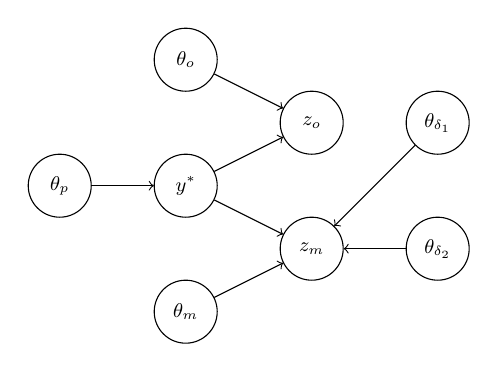
\begin{tikzpicture}[scale=0.8,every node/.style={transform shape}]
%[inner sep=1mm] 
[line width=1pt]
\path (2,0) node (thetap) [shape=circle,minimum size=1cm,draw] {\small $\theta_p$};
\path (4,0) node (ystar) [shape=circle,minimum size=1cm,draw] {\small $y^*$};
\path (6,1) node (zo) [shape=circle,minimum size=1cm,draw] {\small $z_o$};
\path (4,2) node (thetao) [shape=circle,minimum size=1cm,draw] {\small $\theta_o$};
\path (6,-1) node (zm) [shape=circle,minimum size=1cm,draw] {\small $z_m$};
\path (4,-2) node (thetam) [shape=circle,minimum size=1cm,draw] {\small $\theta_m$};
\path (8,1) node (thetad1) [shape=circle,minimum size=1cm,draw] {\small $\theta_{\delta_1}$};
\path (8,-1) node (thetad2) [shape=circle,minimum size=1cm,draw] {\small $\theta_{\delta_2}$};

\draw [->] (thetap) to (ystar);
\draw [->] (thetao) to (zo);
\draw [->] (ystar) to (zo);
\draw [->] (ystar) to (zm);
\draw [->] (thetam) to (zm);
\draw [->] (thetad1) to (zm);
\draw [->] (thetad2) to (zm);
\end{tikzpicture}
\end{figure}

\noindent \cite{McMillan_2010} used an identical framework, (albeit with inference at an aerial resolution and with no $\delta_2$) to combine data from monitoring sites with the Community Multi-scale Air Quality (CMAQ) model output to provide estimates on PM$_{2.5}$ particulate matter. Here the process model was a generic, separable space-time model with spatial precision matrix given by the CAR(1) model \citep{Rue_2005} and the temporal covariance by the AR(1) process. A more elaborate version which facilitates inference at the point-scale is given by \cite{Sahu_2010}. Obviously multiple observation sources can be included, see for instance \cite{Smith_2007}. 

The works mentioned so far all use black-box process models which are flexible so as to accommodate both the observed data and the model output. Mechanistically motivated models, do however frequently appear in this context; for example in \cite{Milliff_2011} where scatterometer data ($z_o$) is integrated with weather forecasts to obtain estimates of the surface-vector winds. Finally we note that in some cases, model outputs may be used to also induce secondary Level 2 process priors, in this case Bayesian melding \citep{Poole_2000} would be necessary to elicit a single process model prior.  The multi observation approach is frequently used in combining climate model output predictions, see Example 4 in Appendix A.

Multi-observation models provide a neat way for assimilating multiple data sets (from models or/and observations) together and despite serving the same goal is conceptually much simpler than the model-informed prior approach. The subtle, yet important distinction to the former approach is that since the model output is expressed in terms of the process we can deal with problems such as change of support \citep{Wikle_2005} with ease (for example, we can say that the model output is an \emph{averaged} version of the true process). However methods in this category are fully focused on realisations and not on the tuning/calibration parameters used to generate the model outputs; these frequently do not feature at all within the framework.  



\section{Data-feature assimilation}

In this section we consider a suite of methods which are selective in their dependence on the underlying physical model, whilst not being as detached from the physical mechanisms as multi-observation approaches (\ref{sec:mo}) and not relying too heavily on the simulator outputs \emph{talis qualis} (Section \ref{sec:mip}). There are cases where the latter would be counter-productive in assimilation: 
\begin{enumerate}
\item When the simulator output is either not reliable, or very hard to validate. This is, unfortunately, the case for natural processes which are also poorly observed such as solid-earth processes or those occurring in the deep ocean or in remote areas of the world such as Antarctica \citep{Guo_2012}. 
\item When the numerical model contains several tuning parameters which are unidentifiable (cannot be calibrated). This is the case for example when treating surface mass balance anomalies in Antarctica, where the anomaly is taken with respect to a long-term \emph{balance state} which is unknown and in all probability highly unstructured spatially. 
\end{enumerate}
In both cases, frequently specialists themselves would be the first to acknowledge that the output and associated uncertainties could be highly inaccurate -- indeed in this case it is debatable whether a data assimilation procedure should at all be used and a data-driven solution might be the appropriate way forward for inference, unless we are faced with under-determined problems such as that discussed next. 

\subsection{Source separation in environmental systems}

For complex physical systems which we deal with, and in particular with interacting systems, fully data-driven approaches (using empirical methods or full Bayes) are not always possible. Consider for example the simple scenario
\begin{equation}\label{eq:problem}
z_o = y_1 + y_2 + e
\end{equation}
\noindent where $z_o$ are experimental observations and a priori $y_1,y_2 \sim \mathcal{N}(0,{\Sigma})$ and $e$ is uncorrelated white noise. Here the unobserved $y_1$ and $y_2$ are confounded (in fact (\ref{eq:problem}) is a saturated collection of co-linear relationships) and whatever the observation coverage, a posterior these two fields are fully sensitive on the prior. In this case one might argue that incorporating a numerical model output to set the prior on at least one of the latent processes might be the best option for data assimilation. However, using the above methods, models with potential substantial discrepancy might not be conducive to the inferential task. 

The source separation problem is a natural generalization of the treatment of \cite{Hodges_2010} who considered the related model
\begin{equation}\label{eq:problem2}
\yvec = \beta \dvec + \xvec + \evec
\end{equation}

\noindent where $\beta$ is an unknown parameter, $\dvec$ is a fixed effect, $\xvec$ is the latent process and $\evec$ has precision $\tau\Imat$. In spatial applications, the precision matrix $\Qmat = \Sigma^{-1}$ is frequently sparse and neighbourhood dependent, so that $\xvec$ usually defines a Gaussian Markov Random Field (GMRF) or conditionally autoregressive prior. Degenerate $\Qmat$ is used for intrinsic versions, these will not be discussed here.  Unidentifiability of $\beta$ in this problem stems from co-linearity between $\dvec$ and the spectral components of $\xvec$, obtained through the decomposition $\Qmat = \Zmat \Lambda \Zmat^T$ where $\Zmat$ is the eigenvector matrix and $\Lambda$ is diagonal with elements corresponding to the eigenvalues of $\Qmat$. The equivalent model
\begin{equation}
\yvec = \beta \dvec + \Zmat \bvec + \evec
\end{equation}
has an implicit prior on $\bvec$ centred on zero with variances inversely proportional to the eigenvalues $\Lambda$. Higher variances would be attributed to the lower frequency components, whilst lower variances (smaller orders of magnitude) with the higher frequencies. Colinaerity between $\dvec$ and columns of $\Zmat$ can drastically (adversely) alter the posterior estimate of $\beta$, both in mean and variance. 

Consider again (\ref{eq:problem}). Now $\yvec  = \Zmat_1 \bvec_1 + \Zmat_2 \bvec_2 + \evec$ where we have assumed that $\xvec_1$ and $\xvec_2$ have different prior distributional properties. It is interesting to see how the Bayes update behaves in this case. For simplicity assume that $\Zmat_1 \equiv \Zmat_2 = \Zmat$ (for practical purposes, highly co-linear) but that $\Lambda_1 \ne \Lambda_2$, then it can be shown (Appendix B) that 
\begin{equation}
var(b^i_1 | \yvec) = \frac{\lambda^i_2 + \tau}{\lambda^i_1\lambda^i_2 + \tau(\lambda^i_1 + \lambda^i_2)} 
%\expect[b^i_1 | \yvec]/\expect[b^i_2 | \yvec] =\frac{\lambda^i_2 + \tau(1 - v^i)}{\lambda^i_1 + \tau(1- v^i)}
\end{equation}
\noindent which, under the prior assumption of spectral similarity ($\lambda^i_1 \equiv \lambda^i_2 = \lambda^i$) will have a lower-bound ($\tau \gg \lambda^i$) of $1/2\lambda^i$. This will not result in informative assessments on the marginals, in general, unless highly informative priors are set on both fields. Thus one would wish the spectral properties to differ a priori. For instance, by setting $\lambda_2^i \gg \lambda_1^i$, the lowerbound is given by the first term on the RHS in
\begin{equation}
var(b^i_1 | \yvec) = \frac{1}{\lambda^i_1 + \tau} + O(1/\lambda_2^i)
\end{equation}
\noindent which is also the standard Gaussian update in the absence of confounded fields. 

The statistician is therefore tasked with finding prior distributions for $\xvec_1$ and $\xvec_2$ which have dissimilar spectral properties, a task which may be aided with simulator outputs. Selectively setting spectral properties corresponds to strategically choosing a set of constraints from simulator data using, for instance, four strategies outlined in Sections 3.3--3.6. 

%Data-feature assimilation provides an all-important strategy in setting our prior spectral characteristics and thus aid uncertainty reduction on the posterior estimates. 




%In this work we show how to use other aspects of the numerical model within the framework, namely by specifying a Level 3 model on selected components from the simulator outputs which define \emph{features} deemed representative by the specialist. Despite its potential, this type of assimilation is remarkably rare in the environmental literature, although there are some isolated works which we will refer to throughout the ensuing discussion.

\subsection{Model setup}

From now on we shall assume that our domain of interest is $\svec \in \mathcal{O}$ where $\mathcal{O} \subset \mathbb{R}^d$. Denote the process as  $y^*(\svec): \mathbb{R}^d \rightarrow \mathbb{R}$. Under the assumption of observations with normally distributed errors, our Level 1 observation model is 
\begin{equation}
z_o(\svec_i) = y^*(\svec_i) + e_{o,i}, ~~~~ i = 1\dots m
\end{equation}
\noindent where $e_o$ is uncorrelated white noise with precision $\tau$ and $m$ is the number of observations. Note that $y^*(\svec_i)$ need not be normally distributed, in general, although this is assumed throughout. Then $\yvec^* = [y^*(\svec_i), y^*(\svec_2), \dots, y^*(\svec_m)]$ is the record of physical observations. 

%Consider now a simulator $f(\svec,\varthetab_m)$. Then, we recall that the basic model-informed prior approach is to let
%\begin{equation}
%y^*(\svec_i) = f(\svec_i;\thetab_m) + \delta(\svec_i) + e_{y,i}, ~~~~ i = 1\dots m
%\end{equation}
%\noindent where $\delta(\svec_i)$ is a discrepancy term. $\delta(\svec)$ needs to be modelled itself, and frequently insight of what constitutes $\delta(\svec)$ needs to known and included appropriately. In this section we are concerned with cases where  either $\delta(\svec)$ is hard to construct from the available simulator outputs, or else too flexible for $f(\svec_i,\thetab_m)$ to impart knowledge on $ y(\svec_i)$ with the number of observations available. 
%
%The approach is similar to the use of the discrepancy in that we assume that the model output is spatially biased from the truth in some way. However we do not enforce a prior model on $\delta(\svec)$. 
The approach rests on constructing a prior distributions for $y^*(\svec)$ and a stationary distribution for the model outputs which are related through a set of constraints. As we shall see this is a very flexible framework and is ideal when the discrepancy is highly unstructured (or unknown) and only certain output features of the numerical model are deemed correct. The basic premise is to represent the true field, and that generated by simulators by stochastic models which share commonalities on a subset of their hyper-parameters (resulting in a selective borrowing of strength). In a Gaussian setting, the model is as follows
\begin{align}
z_o(\svec_i) &\sim \mathcal{N}( y(\svec_i),\tau^{-1}) \\
y^*(\svec) &\sim \mathcal{GP}_1(\svec;\gammab_m,\gammab_c), \\
%\expect_\varthetab[y(\svec,\varthetab)] &\sim \mathcal{GP}_2(\svec;\gammab_t,\gammab_c) 
y(\svec) &\sim \mathcal{GP}_2(\svec;\gammab_t,\gammab_c) 
\end{align}
\noindent with graphical model

\begin{figure}[h!]
\centering
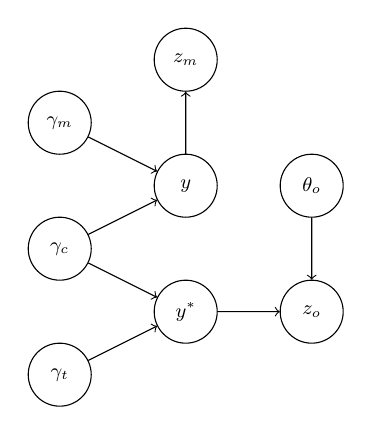
\begin{tikzpicture}[scale=0.8,every node/.style={transform shape}]
%[inner sep=1mm] 
[line width=1pt]
\path (2,4) node (gammam) [shape=circle,minimum size=1cm,draw] {\small $\gamma_m$};
\path (2,0) node (gammat) [shape=circle,minimum size=1cm,draw] {\small $\gamma_t$};
\path (2,2) node (gammac) [shape=circle,minimum size=1cm,draw] {\small $\gamma_c$};
\path (4,3) node (y) [shape=circle,minimum size=1cm,draw] {\small $y$};
\path (4,5) node (zm) [shape=circle,minimum size=1cm,draw] {\small $z_m$};
\path (4,1) node (ystar) [shape=circle,minimum size=1cm,draw] {\small $y^*$};
\path (6,1) node (zo) [shape=circle,minimum size=1cm,draw] {\small $z_o$};
\path (6,3) node (thetao) [shape=circle,minimum size=1cm,draw] {\small $\theta_o$};

\draw [->] (gammam) to (y);
\draw [->] (gammac) to (y);
\draw [->] (gammac) to (ystar);
\draw [->] (gammat) to (ystar);
\draw [->] (ystar) to (zo);
\draw [->] (thetao) to (zo);
\draw [->] (y) to (zm);
\end{tikzpicture}
\end{figure}

\noindent where $\gammab_m$ are model-parameters which are believed to be \lq wrong\rq~in the sense that they impart information on $y^*$ that would be substantially different from if they were equal to  $\gamma_t$. $\gamma_t$ are the \lq true\rq~version of $\gamma_m$ and $\gamma_c$ are parameters believed to be common to both models. 

%There are subtle yet significant differences to when a stochastic model (or a set of) are used to characterise $y(\svec,\varthetab)$ and $\delta(\svec)$ separately. First, unlike e.g. \cite{Higdon_2004}, we do not necessarily need to assume that all hyper-parameters of $\mathcal{GP}_2$ are representative of the truth. Further, we are not concerned with retaining dependency on $\varthetab$ as the complex nature of $\delta(\svec)$ is such that the model output, in the cases we are interested in, is itself not of use. The variability of the features in $\gammab_m$ which arise due to uncertainty in the parameters could be informative however.  Finally, the primary purpose of the exercise is assimilation and not prediction, obviating the need for a reliable parameter model and an estimate of the best parameter $\thetab_m$. 


% Note, however, that we do not constrain RP to be a Gaussian process as there are several interesting cases when this need not be the case. 

\subsection{Incorporation of frequency characteristics}

In the first example of this approach we consider the case where thre is confidence on the spectral decomposition of the output ensemble, but not on the output values themselves. This is the case for instance when models are still in their early stage of development, or when the output depends on some variable which is unknown and cannot be observed (e.g.~the long-term climate mean mentioned earlier). The model for this case is given as
\begin{align}
y(\svec) &\sim \mathcal{GP}_1(\mu(\svec;\gammab_m), k(\svec,\rvec;\gammab_c)), \\
y^*(\svec) &\sim \mathcal{GP}_2(\mu(\svec;\gammab_t), k(\svec,\rvec;\gamma_c))
\end{align}
\noindent where $\mathcal{GP}(\mu,k(\cdot,\cdot))$ denotes a Gaussian process with mean $\mu$ and covariance function $k$. 

This scenario equates to using model outputs to configure spectral filters with which to use on the data. To see this assume that we have a few observations $\zvec_o$ at isolated points $\svec$. If the covariance kernel $k(\svec,\rvec)$ is a Mat{\'e}rn kernel of the form
\begin{equation}\label{eq:Matern}
k(\svec,\rvec) = \frac{\sigma^2}{2^{\nu-1}\Gamma(\nu)}(\kappa\| \svec - \rvec \|)K_\nu(\kappa\| \svec - \rvec \|),
\end{equation}
\noindent then prior to regression (in an empirical setting), one might first obtain point estimates for $\nu, \sigma^2$ and $\kappa$. By the auto-covariance theorem, which states that the Fourier transform of the auto-covariance function of the GP is the power spectral density of the signal, this is an implicit estimation of the signal spectral characteristics. For the Mat{\'e}rn, the spectral density is 
\begin{equation}
R(\kvec) \propto (2\pi)^{-d}(\kappa^2 + ||\kvec||^2)^{-\alpha}, ~~~ \alpha = \nu + d/2
\end{equation}
\noindent where $d$ is the spatial dimensionality. When observations are sparse, information on the hyperparameters govering the spectral density is poor. However there is valuable information in the numerical models which can be used. Thus, in this framework one imposes  that the hyper-parameters describing the covariance of $y(\svec,\tvec)$ and $y^*(\svec)$ are the same i.e. $\gammab_c = \{\nu, \sigma, \kappa\}$. Note that we are not informing the prior mean of $y^*(\svec)$ through the model outputs as is done in standard data assimilation, nor are we treating the model output as data which would thus inevitably also alter the posterior conditional mean with respect to the fully data-driven approach.

%For illustration of this approach we generate two realizations from a Gaussian process and treat one as the real system and one as the model output. We then generate 10 equally spaced observations with standard deviation $\sigma = 0.5$ and estimate the hyperparameters (using a simple grid search in this problem) for the three options $\nu \in \{ 1/2, 3/2, 5/2\}$. For the problem in Fig. \ref{fig:GPtests} these are estimated as $\hat\nu = 5/2, \hat\sigma = 2.26, \hat \kappa = 0.26$ (the true values were $\hat\nu = 1/2, \sigma = 2, \hat \kappa = 0.1$). Note how the regressed curve (and associated uncertainty intervals) are overly smooth, and fails to capture variability of the true process. This would not be picked up using standard cross-validation techniques if our problem was defined by (\ref{eq:problem}).  We next re-do the exercise by first tuning the hyper-parameters based on the numerical model output. This now gives $\hat\nu = 1/2, \hat\sigma = 1.34, \hat \kappa = 0.31$. Note how the uncertainty intervals are now widened to cater for the lack of smoothness. The frequency-response estimated from the data and that from the numerical model are shown in Fig. \ref{fig:GPtests} together with that of the true process.
%
%\begin{figure*}[t!]
%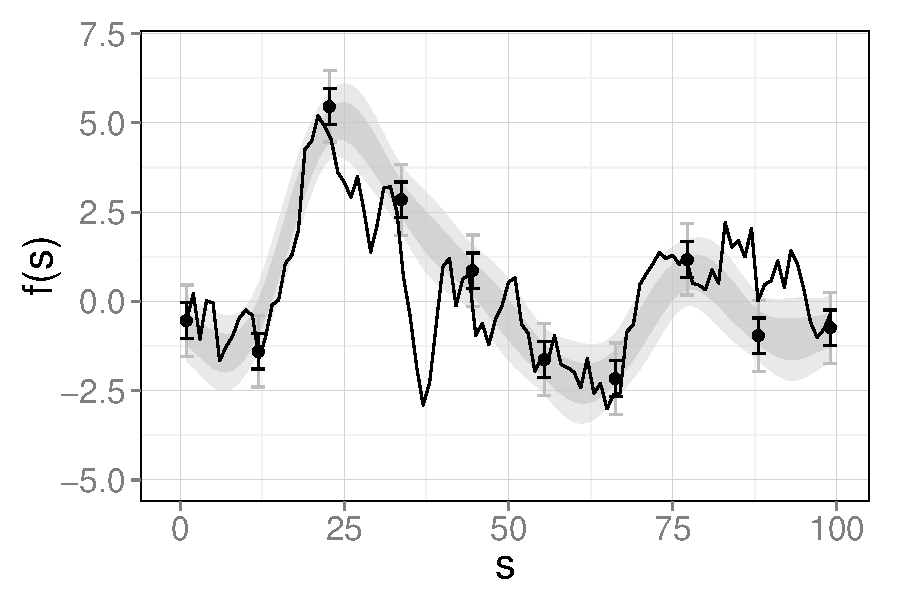
\includegraphics[width=2.8in]{GP1.pdf}
%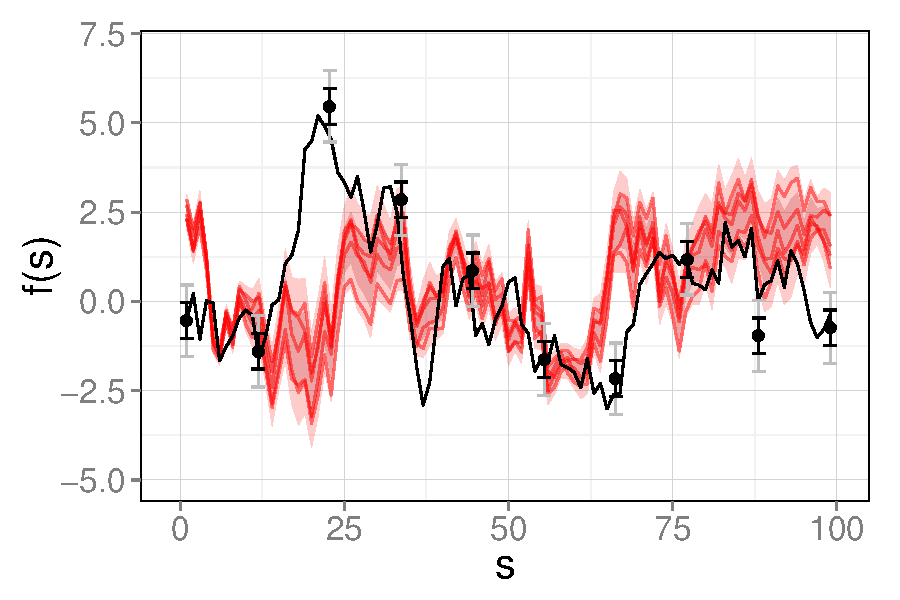
\includegraphics[width=2.8in]{GP2.pdf} \\
%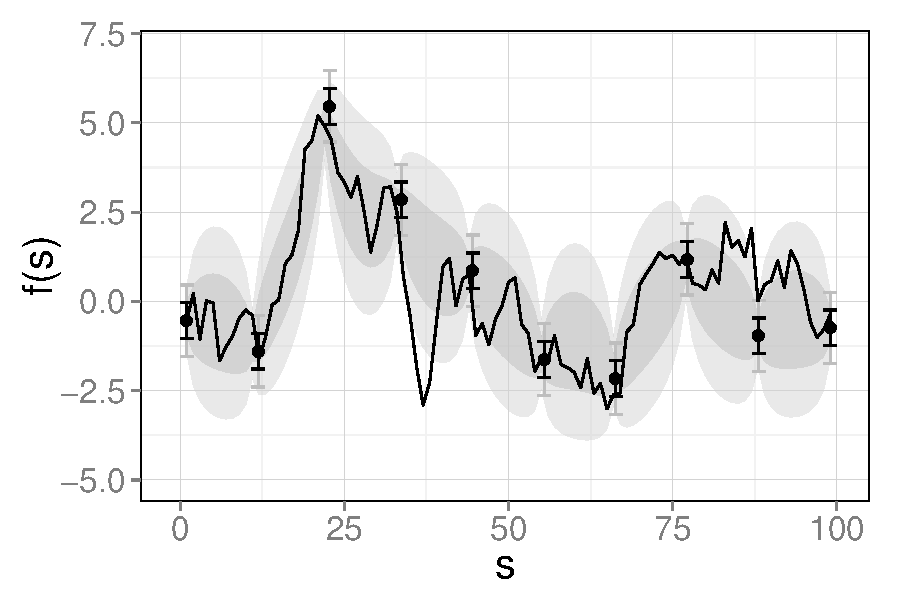
\includegraphics[width=2.8in]{GP3.pdf}
%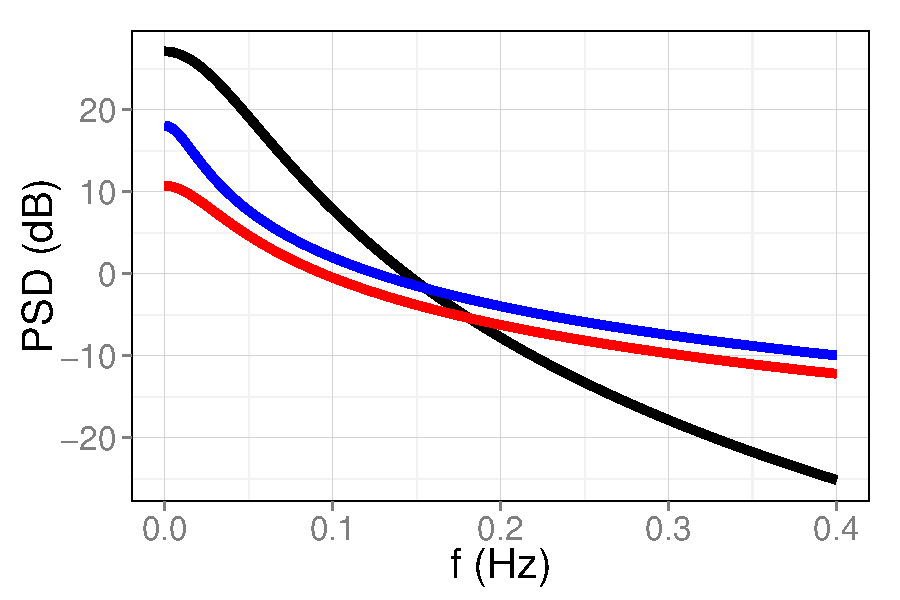
\includegraphics[width=2.8in]{GP4.pdf}
%\caption{Top left: Inference using empirical estimates of $\gamma_c$ from the data. Bottom left:  Inference using empirical estimates of $\gamma_c$ from model outputs. Top right: Truth (solid line), observations (dots with 1$\sigma$ and 2$\sigma$ error bars) and model simulations (red). Bottom right: True power spectrum (solid), power spectrum estmimated from the data (dotted) and from the model (dashed). Note how the high frequencies are under-represented in the data spectrum due to aliasing.}\label{fig:GPtests}
%\end{figure*}

An example of works employing this approach include \cite{Berliner_2000} where the spatial covariance matrix of global mean temperature was estimated from surrogate model output, and \cite{Zammit_2013} where the heterogeneous characteristics of a surface anomaly were extracted from numerical model output and used to set up a prior spatial model.

\subsection{Incorporation of spatial characteristics}

In other cases there is confidence on the spatial patterns (basis functions) of the model output, but not on the magnitude or covariance of these functions. The underlying model in this case is
\begin{align}
y(\svec) &\sim \mathcal{GP}_1(\phi_c(\svec)^T\xvec(\gamma_m),  \phi_c(\svec)^T\Sigma(\gamma_m)\phi(\rvec)), \\
y^*(\svec) &\sim \mathcal{GP}_1(\phi_c(\svec)^T\xvec(\gamma_t),  \phi_c(\svec)^T\Sigma(\gamma_t)\phi(\rvec)), 
\end{align}
\noindent where $\phib_c$ are the basis functions common to both processes, $\xvec$ the respective weights, and where $\Sigma = Var(\xvec)$. 

The most straightforward application of this method is fingerprinting where, for instance, the pattern of CO$_2$ forcings is used as a template to test whether observations support anthropogenic forcings or not. In \citep{Berliner_2000} the fingerprint appears as the \emph{mean} of the temperature anomalies, wieghted by some unknown parameter $a$. The fingerprint can be viewed as a basis function deemed as characteristic to the process of interest. Other cases include \cite{Wikle_2001}, where eigenvectors are estimated from a model describing sea-level pressure, the weights of which are subsequently estimated in assimilation. Constraining the process to lie on a low-dimensional space is beneficial when the observations are sparse and even more so when the low frequencies of two signals are confounded \citep{Zammit_2014}.


\subsection{Incorporation of dynamical information}

Spatio-temporal modelling is a powerful tool extensively employed in environmental applications. Frequently, as in the fixed rank filtering case studies of \cite{Cressie_2010} and \cite{Kang_2010}, dynamic information may be obtained directly from the data \citep[see also][]{Wikle_2002,Dewar_2009}. In other cases this is not plausible, particularly when the observations are \lq patchy\rq~or are highly irregular spatio-temporally. One way to overcome this problem is to extract dynamic information from the model output and using this to inform the true process model $y^*$. For a linear vector Gaussian spatio-temporal model we thus might have
\begin{align}
y_{t+1}(\svec) = [\mathcal{A};\gamma_c]y(\svec)_t + w(\svec;\gamma_m)_t \\
y_{t+1}^*(\svec) = [\mathcal{A};\gamma_c]y^*(\svec)_t + w(\svec;\gamma_t)_t 
\end{align}

\noindent where $\mathcal{A}$ is an operator propagating $y(\svec)_t$ in time and $w(\svec)$ is an additive disturbance. This was the approach taken by \cite{Calder_2011} in modelling the spatio-temporal dynamics of aerosols where $\mathcal{A}$ was the integro-difference operator \citep{Kot_1986} and $\gamma_c$ denoted the (spatially-varying) characteristics of flor direction and dispersion. 

This approach is appealing as algorithms are today becoming available to extract dynamics  .... \red{Botond, can you just write out in a few lines a model for y, how we discretise, and how we estimate Amat and then put a picture of the field (going round in circles) and an estimate of the arrows? Just mention you use EP then we cite the paper on ArXiV.}

\subsection{Incorporation of soft constraints}

\red{Botond, can you also write this out and put in maybe a toy study from what you had in NIPS.}




								


\section{Conclusion}

\bibliography{Assim_bib}

\newpage
%
%\appendix
%\section{Examples}
%
%\paragraph{Example 1: Ensemble Kalman Filtering}
%Ensemble Kalman filtering (EnKF) is the simplest application of the model-informed prior approach approach where $\theta_m$ are the initial conditions at a given time (say $t$). The model ensemble is generated by running the simulator $f(\cdot)$ for a short time period until the next observation at $t+\Delta_t$ for each of the different initial conditions. In EnKF there is no discrepancy term, and all parameters (except $\theta_m$) are assumed known. This implies a one-to-one mapping between $\theta_m$ and $y^*$ so that one of these terms (we choose $\theta_m$) can be omitted in a much simplified graphical model:
%\begin{figure}[h!]
%\centering
%\begin{tikzpicture}[scale=0.8,every node/.style={transform shape}]
%%[inner sep=1mm] 
%[line width=1pt]
%\path (4,0) node (ystar) [shape=circle,minimum size=1cm,draw] {\small $y^*$};
%\path (6,0) node (zo) [shape=circle,minimum size=1cm,draw] {\small $z_o$};
%\draw [->] (ystar) to (zo);
%\end{tikzpicture}
%\end{figure}
%
%\noindent The distribution of the true process $y^*$ is fully determined by that of $\theta_m \sim p_1(\theta_m)$, and is given by
%\begin{equation}
%p(y^*) = p_1(f^{-1}(y^*))\left| \frac{\intd f^{-1}(y^*)}{\intd y^*}\right|
%\end{equation}
%\noindent Equation (\ref{eq:Sim_simple}) reduces to
%\begin{equation}
%p(y^*|z_o) \propto  p(z_o | y^*)p(y^*)
%\end{equation}
%\noindent As earlier we are faced with a very complicated induced distribution due to presence of $f$ which, even if known, need not be invertible. In EnKF the computation is facilitated by approximating the induced distribution as a normal distribution
%\begin{equation}
%y^* \sim \mathcal{N}(\mu_m,\Sigma_m; \theta_m)
%\end{equation}
%\noindent and $\mu_m = \expect[f(\theta_m)]$ and $\Sigma_m = var[f(\theta_m]$ which can be easily found empirically from a small ensemble of, say, 50 runs (details are given later).  
%
%The \lq Kalman filtering\rq~in EnKF refers to the linear, sequential nature of this estimate i.e. $z_o = Cy^* + e$ with $e$ zero-mean Gaussian with covariance $\Sigma_o$ assumed.  The required posterior distribution is then
% \begin{equation}
%   p(y^* | z_o) \propto \exp\left(-\frac{1}{2}(z_o - Cy^*)^T\Sigma_o^{-1}(z_o - Cy^*) - \frac{1}{2}(y^* - \mu_m)^T\Sigma_m^{-1}(y^* - \mu_m) \right) 
% \end{equation}
%\noindent which is normally distributed with precision and mean given by
%\begin{align}
%\Sigma_a^{-1} &= C^T\Sigma_o^{-1}C + \Sigma_m^{-1} \\
%\mu_a &= \Sigma_a[C^T\Sigma_o^{-1}z_o + \Sigma^{-1}_mz_m]
%\end{align}
%\noindent The usual KF equations are obtained by applying the Sherman-Woodbury formula to the precision matrix to yield
%\begin{align}
%\Sigma_a &= (I - KC)\Sigma_m \\
%\mu_a &= z_m + K(z_o - Cz_m) \label{eq:EnKFmean}
%\end{align}
%\noindent where $K = \Sigma_mC^T(\Sigma_o + C\Sigma_mC^T)^{-1}$ is the Kalman gain. Note that for the single model output case (where $\Sigma_f$ needs to be specified using some other means), $\mu_a$ reduces to the 3DVAR estimate \citep{Hamill_2000}.
%
%The \lq Ensemble\rq~ in EnKF refers to the Monte Carlo nature alluded to earlier by which the mean and covariance are computed for when $f(\thetab_m) \in \mathbb{R}^{n \times N}$, where $N$ is the number of model ensembles and $n$ is the state dimensionality (i.e. $\thetab_m$ are $N$ samples from $p(\theta_m)$). The predictive mean is simply $\mu_m = \expect[f(\thetab_m)]$ while the covariance $\Sigma_m$ is estimated as the empirical covariance between the ensemble members as  $\Sigma_m = \expect[(f(\thetab_m) - \expect[f(\thetab_m)])(f(\thetab_m) - \expect[\thetab_m])^T]$. 
%
%The update step is also carried out using these realisations, First an ensemble of pseudo-observations $z_{o,m} \in \mathbb{R}^{m \times N}$ is generated by repeatedly sampling from $\mathcal{N}(z_o,\Sigma_o)$. Then the update (computation of posterior mean) is performed on each member separately to get a set of ensemble means $\mu_{a,m} \in \mathbb{R}^{n \times N}$ referred to as the \emph{analysed estimates}:
%\begin{equation}
%\mu_{a,m} = f(\thetab_m) + K(z_{o,m} - Cz_m)
%\end{equation}
%It can be shown that the mean of these estimates, $\expect[\mu_{a,m}]$, converges to $\mu_a$ in the large sample limit, as does the sample posterior covariance $\expect[(\mu_{a,m} - \expect[\mu_{a,m}])(\mu_{a,m} - \expect[\mu_{a,m}])^T]$ to the true posterior covariance $\Sigma_a$, see \cite{Burgers_1998} for further details.
%
%EnKF is a quick and efficient way for data assimilation. However simulation with $f(\cdot)$ needs to be quick and moreover, the assumptions imposed are strong: $p(y^* | z_o)$ is restricted to be Gaussian (only the mean and covariance of the ensemble members are used), the observation models are linear and the posterior mean is effectively a weighted average of the model outputs and the observations. Full-blown sequential Monte Carlo (SMC) methods may be used to remedy this, however computational issues and degeneracy in high dimensional systems would be problematic. Model bias/discrepancy is not accounted for. Thus EnKF (or any corresponding SMC method) should only be used when the simulator $f(\cdot)$ is reliable, i.e. when observations are sufficiently regular in time so that any disrepancy arising due to $f(\cdot)$ may be safely assumed to be inconsequential.
%
%\paragraph{Example 2: The linear Gaussian emulator} Here we consider a similar case to \cite{Higdon_2004} where $\theta_o$ is known. However to make the example even simpler we assume an emulator which is linear in $\vartheta_m$ and a model output (and hence observation) which is a scalar. For this example we will use bold typeface to denote vectors for clarity. Assume that we have $N$ runs of the full system with inputs $\varthetab_m$ and outputs $\zvec_m$. The full system equations are as follows:
%\begin{align}
%\zvec_o &= \yvec^* + \evec_o,~~~~ \evec_o \sim \mathcal{N}(0,\Sigma_o) \\
%y^* &= y(\theta_m) + \delta,~~~~ \delta \sim \mathcal{N}(\mu_\delta,\sigma^2_\delta) \\
%y(\vartheta_m) &= \beta\vartheta_m + e_y,~~~~ e_y \sim \mathcal{GP}(0,k(\vartheta_m,\vartheta_m';\theta_p')) \\
%\zvec_m &= y(\varthetab_m) + \evec_m, ~~~~ \evec_m \sim \mathcal{N}(0,\Sigma_m)
%\end{align}
%\noindent where we let $\theta_\delta = (\mu_\delta,\sigma^2_\delta)$, $\theta_p = (\beta,\theta_p')$ and assume that $\theta_p'$ is independent of $\vartheta_m$ although this can be relaxed in practice (for example the variance is linearly related to $\vartheta_m$). The quantity $\Sigma_m$ is typically diagonal and reflects the small-scale error in emulator construction (also the nugget effect in kriging). The model outputs act as training data; the corresponding process values at $\varthetab_m$ are $\yvec = y(\varthetab_m)$. 
%
%In this first stage it is required to find the posterior distribution of $y$ at a particular point $y(\theta_m)$, this is a classical problem in Gaussian process prediction \citep{Rasmussen_2006}. A trick to simplify computations in GP prediction is to directly consider the \emph{joint} distribution
%\begin{equation}
%p(\zvec_m,y^* | \theta_m,\varthetab_m) \propto \int p(\zvec_m,y^* | \yvec, \theta_m,\theta_\delta)p(\yvec | \varthetab_m,\theta_p)p(\theta_p) \intd \theta_p \intd \theta_\delta\intd \yvec
%\end{equation}
%\noindent If we can somehow fix $\theta_p,\theta_\delta$ (using, for instance empirical methods such as trend analysis and semivariograms, or at each sample in an MCMC scheme), then this distribution reduces to
%\begin{equation}
%p(\zvec_m,y^* | \theta_m,\varthetab_m) \propto \mathcal{N}\left(\begin{bmatrix}\beta\varthetab_m \\ \beta\theta_m + \mu_\delta \end{bmatrix},\begin{bmatrix} \Sigma_m + \Sigma_{\varthetab_m} & \Sigma_{\varthetab_m\theta_m} \\ \Sigma_{\theta_m\varthetab_m} & \sigma^2_{\theta_m} + \sigma^2_\delta \end{bmatrix}  \right)
%\end{equation}
%\noindent where $\Sigma_{\varthetab_m} = k(\varthetab_m,\varthetab_m)$ and $\Sigma_{\varthetab_m\theta_m} = k(\varthetab_m,\theta_m)$. By Gaussian conditioning we can then find $p(y^* | \zvec_m,\theta_m,\varthetab_m)$ as 
%\begin{align}
%p(y^* | \zvec_m,\theta_m,\varthetab_m) = \mathcal{N}(\Sigma_{\theta_m\varthetab_m}[\Sigma_{\varthetab_m\varthetab_m} &+ \Sigma_m]^{-1}(\zvec_m - \beta \varthetab_m) , \\
%&\Sigma_{\theta_m\theta_m} - \Sigma_{\theta_m\varthetab_m}[\Sigma_{\varthetab_m\varthetab_m} + \Sigma_m]^{-1}\Sigma_{\varthetab_m\theta_m})
%\end{align}
%\noindent The next stage is to find $p(y^* | \zvec_o, \zvec_m, \theta_m, \varthetab_m) \propto p(\zvec_o | y^*)p(y^* | \zvec_m,\theta_m,\varthetab_m)$, a simple Guassian update which also results in closed form expressions for a given $\theta_m$. Now all that remains is to marginalise out $\theta_m$ which, even in this simplest of cases, will require sampling due to the complicated nature with which this variable appears in the problem (in machine learning terms, as a random  \emph{test point}). However sampling this posterior is very quick, unlike in the former case when $f(\vartheta_m)$ is repeatedly evaluated. In this case the effective dimensionality is only as large as the dimensionality of $\theta_m$, in practice parameters $\theta_p, \theta_o$ and $\theta_\delta$ will also need to be sampled. An alternative to sampling in a full Bayesian approach shown here is to use Bayes linear adjustments, see \cite{Craig_2001}.
%
%\demo
%
%\paragraph{Example 3: First-order emulation} Another alternative to lowering the computational burden is to create a simple structure for the emulator, such that it only captures the first-order characteristics in the model parameter space. This approach has been gaining interest recently in ecological applications \citep{Hooten_2011,Leeds_2013}. \red{Bill can you right about a simple first-order linear emulator? Maybe you just need to allude at nonlinear models/random forests at the end (I still need to get to grips with random forests!) Maybe also mention polynomial chaos stuff which I think falls into this class (e.g.Jann Paul Mattern 2013)? As you wish.}. 
%
%
%\paragraph{Example 4: Combining climate model output predictions:} The multi-observation approach lends itself nicely to combining several model outputs from different climate simulators in the Coupled Model Intercomparison Project (CMIP). As a case study we consider \cite{Furrer_2007}. Here the model outputs of interest are spatial average temperatures at grid locations and each of the $N$ models is associated with its own observation model given as $z_o^i = Cy_i + \epsilon_i$ where $C$ maps the spherical harmonics weights $y_i$ to the data and $e_i$ reflects the small-scale signal error. The model weights $y_i$ are modelled as $y_i = y + v_i$ where $v_i$ is uncorrelated noise, i.e. the model spherical harmonic weights are assumed to be unbiased versions of the truth. A discrepancy term is implied, as seen by substituting $y_i$ into the observation model to obtain
%\begin{equation}
%z_o^i = Cy + \delta_1 + e_i
%\end{equation}
%\noindent where $\delta_1 = Cv_i$ is the large-scale discrepancy. The process model is taken to simply be $y \sim \mathcal{N}(0,\eta)$ where $\eta$ is set so that the prior is uninformative. The ensuing graphical model for this specific scenario is as follows
%\begin{figure}[h!]
%\centering
%\begin{tikzpicture}[scale=0.8,every node/.style={transform shape}]
%%[inner sep=1mm] 
%[line width=1pt]
%\path (0,0) node (y) [shape=circle,minimum size=1cm,draw] {\small $y$};
%\path (2,1) node (zm1) [shape=circle,minimum size=1cm,draw] {\small $z_m^1$};
%\path (0,2) node (thetam1) [shape=circle,minimum size=1cm,draw] {\small $\theta_m^1$};
%\path (2,-1) node (zmN) [shape=circle,minimum size=1cm,draw] {\small $z_m^N$};
%\path (0,-2) node (thetamN) [shape=circle,minimum size=1cm,draw] {\small $\theta_m^N$};
%\path (4,1) node (thetad1) [shape=circle,minimum size=1cm,draw] {\small $\theta_{\delta_1}$};
%\path (4,-1) node (thetadN) [shape=circle,minimum size=1cm,draw] {\small $\theta_{\delta_N}$};
%
%
%\draw [->] (thetam1) to (zm1);
%\draw [->] (y) to (zm1);
%\draw [->] (y) to (zmN);
%\draw [->] (thetamN) to (zmN);
%\draw [->] (thetad1) to (zm1);
%\draw [->] (thetadN) to (zmN);
%
%\draw [loosely dashed] (zm1) to (zmN);
%\draw [loosely dashed] (thetad1) to (zm1);
%\draw [loosely dashed] (thetadN) to (zmN);
%\end{tikzpicture}
%\end{figure}
%
%\noindent This framework is related to the Reliability Ensemble Average approach where each model is weighted according to its reliability (given through the variance of $\epsilon_i$) which may be estimated empirically \citep{Giorgi_2002}. Note that a present-day observation model can be easily included in this model setup \citep[see also][]{Smith_2009,Tebaldi_2007}. A more elaborate version of the example given here including space-time dynamics is given in \cite{Berliner_2008}.
%
%\demo


\end{document}



